% !TEX root = ./../../_Thesis.tex

% section's Name and Label
\section{Optics and Wavefront Theory}
\label{sec:OpticsAndWavefrontTheory}

The human eye consists of several optical components, notably the cornea, the crystalline lens, the pupil, and the retina. Visual aberrations are the combination of the imperfections/anomalies from the outermost  to the innermost  component. The aim of vision correction is to remove or to minimize the ocular aberrations of the visual system. But to achieve this goal, we first need to understand and analyze how light behaves inside the eye.

%There are two main aspects to how human eye forms images. One is concerned with the physics of image formation and the other with its geometry. We need the former's approach to determine how light waves propagate and behave in the eye, or optical system in general. The geometrical one is a linear interface based on the simplified directional model of light propagation. However, 
According to \citet{Sacek2015} even though \emph{geometrical optics} provides a proper way of determining image location and magnification by tracking paraxial rays, the determination of optical systems' aberrations require more complex calculation considering light waves and its propagation (\ie, \emph{physical optics}).

% O paragrafo e a figura abaixo estão deslocados, sem aparente conexao com o restante do texto
%
%In Figure~\ref{fig:reduced_eyes} it is possible to see two very useful schematic eye models, which allows for a very simple calculation of the refracting power of the entire eye. Both are based in the most influential schematic eye model, constructed by Nobel Laureate Allvar Gullstrand (REF???), and can be used widely used either in geometrical or physical optics.
%
%\begin{figure}[b]
%
	%\centering
	%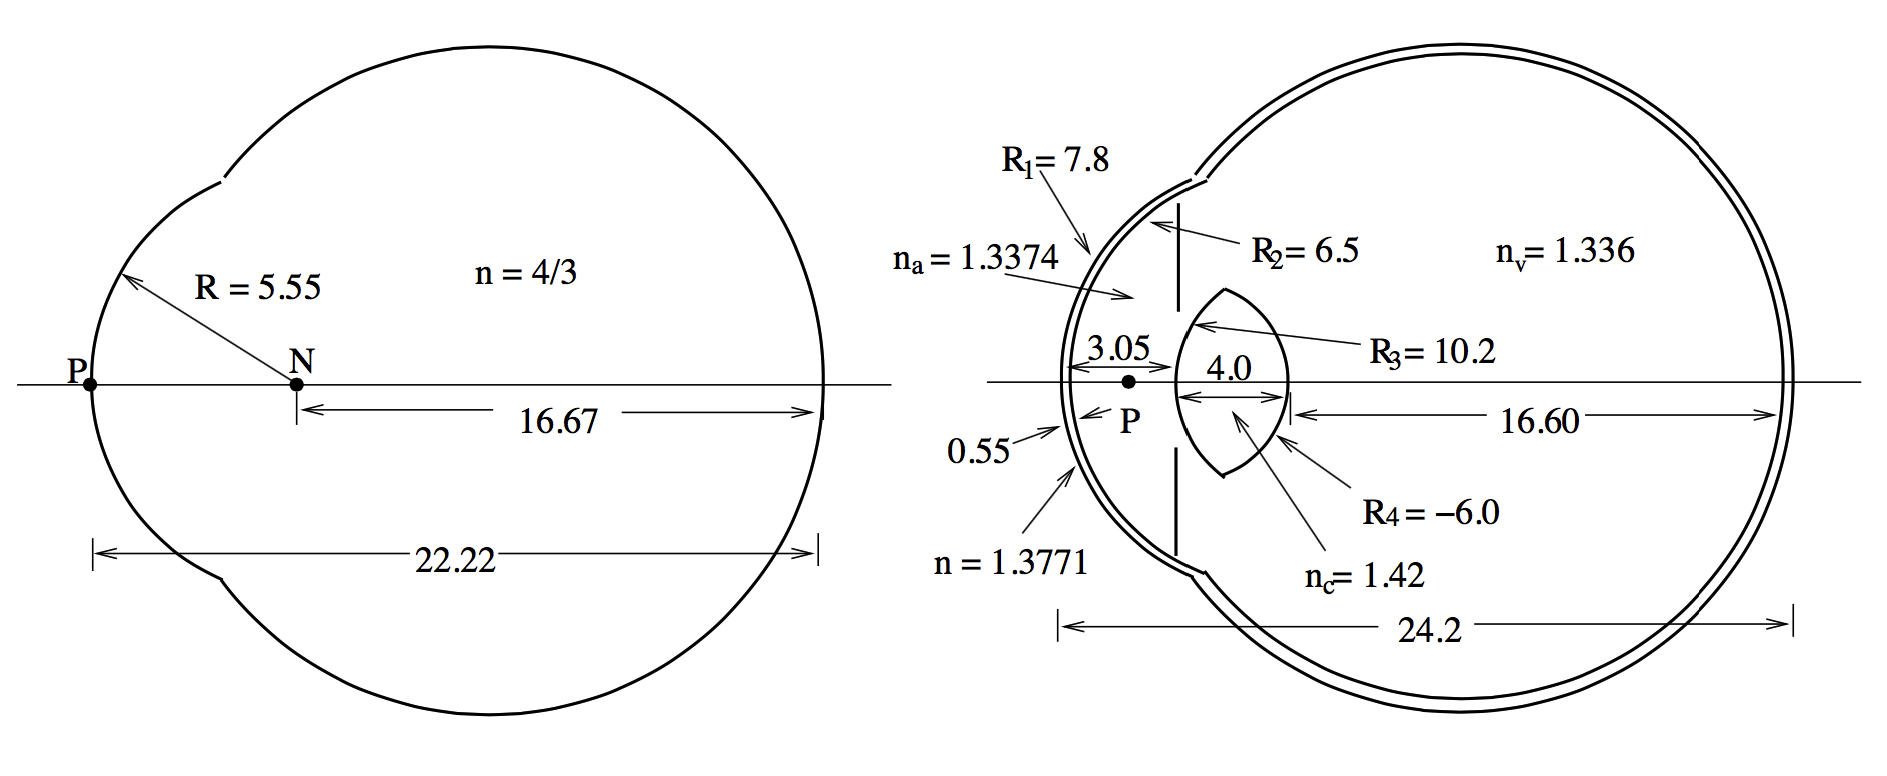
\includegraphics[width=0.95\linewidth]{__Images/02/schematic_eyes.png}
	%\caption[Two very useful schematic eye models]{Two very useful schematic eye models: (right) Emsley reduced schematic eye; (left) Gullstrand-Le Grand theoretical eye. All distance measures are in mm \cite{Dai2008}.}
	%\label{fig:reduced_eyes}
%\end{figure}


\citet{Dai2008} states that "a propagating wavefront can be characterized as many rays propagating in different directions as determined by the local slopes of the wavefront surface". Suppose there is an original wavefront $W(x,y)$, centered at point $O$ and conformed within the aperture $\Sigma$, as shown in Figure~\ref{fig:wavefront_geometry}. When it propagates towards an eye by a distance $d$, it becomes a new wavefront $W'(x',y')$ given as

\begin{equation}
	\centering
	\label{eq:propwave}
	W'(x',y') = W(x,y) + z(x,y;x',y'),
\end{equation}
%	z(x,y;x',y') = \sqrt {d^2+(x-x')^2+(y-y')^2}
\noindent
where $z(x,y;x',y')$ is the distance between points $P(x,y)$ and $P'(x',y')$ (Figure~\ref{fig:wavefront_geometry}), and can be written as:
\begin{equation}
	\centering
	\label{eq:dist}
	z(x,y;x',y') = \sqrt {d^2+(x-x')^2+(y-y')^2}.
\end{equation}

\begin{figure}[!t]

	\centering

	\subfigure[]{
		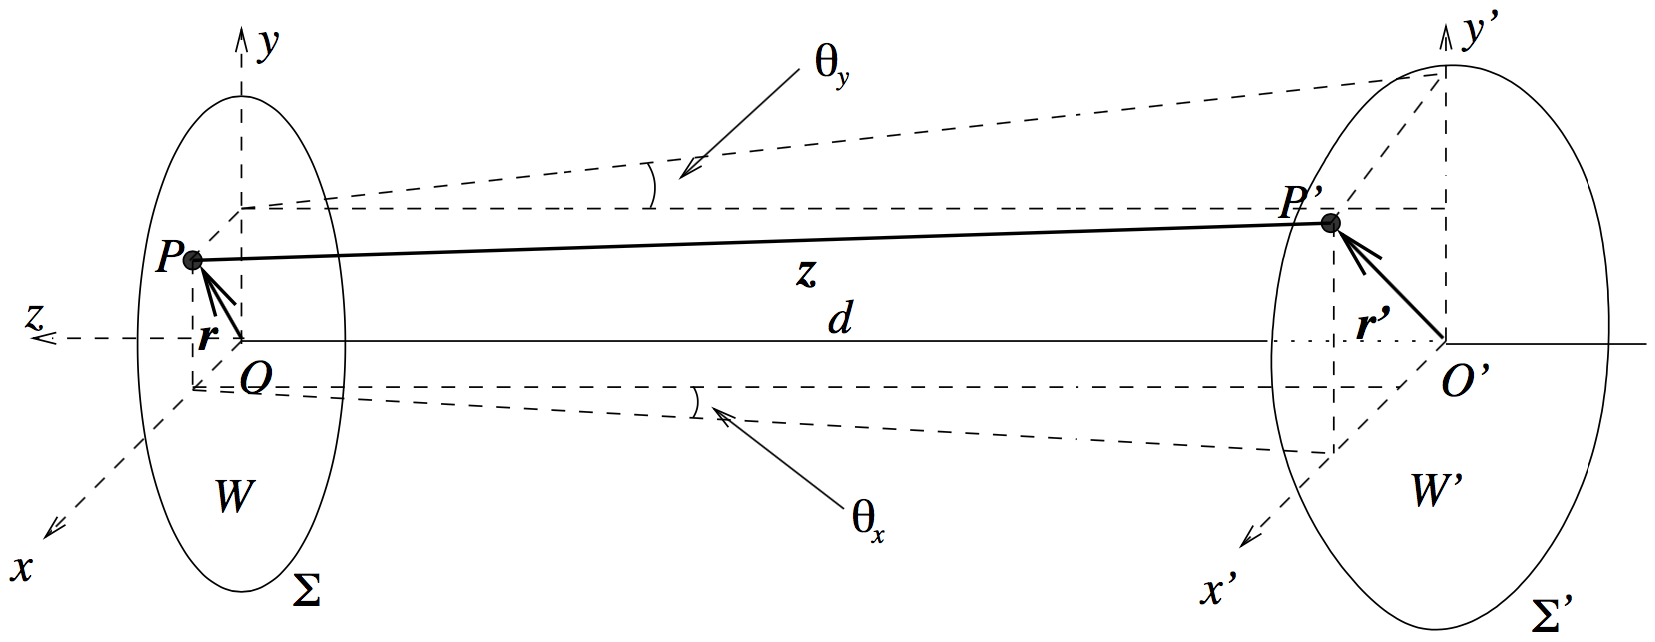
\includegraphics[width=0.7\linewidth]{__Images/02/wavefront_geometry.png}
		\label{fig:wavefront_geometry}
	}
	~
	\subfigure[]{
		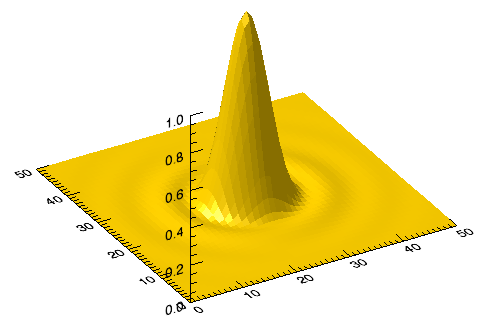
\includegraphics[width=0.25\linewidth, height=10em]{__Images/02/psf_airy3d.png}
		\label{fig:psf_geom}
	}

	\caption[General concepts of wavefront]{General concepts of wavefront: (a) Geometry of the wavefront propagation \cite{Dai2008}; (b) the PSF generated by an aberrated wavefront \cite{Smith2015}.}
	\label{fig:wave_psf}
\end{figure}

The propagation of a wavefront $W(x,y)$ consisting of low-order aberrations only, expressed with Zernike Polynomials, is discussed by \cite{Dai2008}. In addition, the author discusses several optical metrics of ocular wavefronts. A very good predictor for visual performance is the point spread function (PSF), which describes how a ray of light is dispersed in a given space. It is represented by a 2-D array and, as shown in Figure~\ref{fig:psf_geom}, resembles a surface in 3-D. It can be obtained using Fourier Optics \cite{Goodman2005} and the eye's wavefront aberration information. 
% and then used as a 2-D blur filter to be convolved with an image.

\section{Summary}
%
This chapter reviewed the background information about the human eye required for understanding the remaining of this thesis. 
